\subsection{Auxiliary Predicates}

%----------------------------------
\subsubsection{At the intersection}
\begin{center}
    $ atTheIntersection(V) \; \leftrightarrow \; \Big(  arrived(V) \; \land \; \neg entered(V) \Big) $
\end{center}
where
\begin{center}
    $ arrived(V) \; \leftrightarrow \; (\exists F)(\exists T) arrivedAtForkAtTime(V, F, T) $
\end{center}
and
\begin{center}
    $ entered(V) \; \leftrightarrow \; (\exists F)(\exists T) enteredForkAtTime(V, F, T) $.
\end{center}
The predicates $arrivedAtForkAtTime$ and $enteredForkAtTime$
represent the events
\emph{arrival at an intersection} and
\emph{entering an intersection}, respectively.
The time parameter $T$ in these predicates
is called a \emph{time stamp}.

%----------------------
\subsubsection{In the intersection}
\begin{center}
    $ inTheIntersection(V) \; \leftrightarrow \; \Big(  entered(V) \; \land \; \neg exited(V) \Big) $
\end{center}
where
\begin{center}
    $ exited(V) \; \leftrightarrow \; (\exists E)(\exists T) exitedFromAtTime(V, E, T) $.
\end{center}

%----------------------
\subsubsection{Arrival precedence}
\begin{center}
    $ arrivedEarlierThan(V1, V2) \; \leftrightarrow $ \\
    $ (\exists T1)(\exists T2) \Big( arrivedAtTime(V1, T1) \; \land $ \\
    $ arrivedAtTime(V2, T2) \; \land \; T1 < T2 \Big).$
\end{center}
where
\begin{center}
    $ arrivedAtTime(V, T) \; \leftrightarrow \; (\exists F) arrivedAtForkAtTime(V, F, T) $.
\end{center}

The $arrivedSameTime$ is similar,
except `$=$' instead of `$<$'.
%----------------------
\subsubsection{On-the-right-of relation for vehicles}
\begin{center}
    $ isOnRightOf(V1, V2) \; \leftrightarrow \; (\exists F1)(\exists F2)(\exists T1)(\exists T2) \Big( $ \\
    $ arrivedAtForkAtTime(V1, F1, T1)\; \land $ \\
    $ arrivedAtForkAtTime(V2, F2, T2) \; \land \; isOnRightOf(F1, F2) \Big).$
\end{center}
The latter $isOnRightOf$ is a static fact between two forks.

%-----------------------------------
\subsubsection{Lane request}
At arriving at an intersection,
a vehicle must communicate (to other vehicles) its path through the intersection.\footnote{In fact, a vehicle must signal starting at 100 feet from the intersection \cite[p. 61]{DMV-California.2019}}
The turn signal is used to communicate that.
We say a vehicle \emph{requests} an intersection-lane using its turn signal.\footnote{Note that
due to the limited communication capacity of a turn signal,
more than one lane may be requested.
For example,
a left-turn signal could mean a U-turn,
or a left-turn to a crossing street.}

An \emph{intersection lane} is a lane
that connects an incoming lane of the intersection to an outgoing lane.
A \emph{fork} is the collection of all intersection lanes from an incoming lane.
Therefore,
an incoming lane uniquely identifies a fork, and vice versa.

Each intersection-lane determines
which turn signal must be used
if a vehicle wants to pass through the intersection using that lane.
That signal is called the \emph{correct signal} for the lane.

Therefore,
a lane $L$ is requested by a vehicle $V$,
if $V$ signaled the correct signal for $L$
when arriving at $L$'s fork $F$:
\begin{center}
    $ requestedLane(V, L) \; \leftrightarrow  $ \\
    $ (\exists S)(\exists F) \Big( signaledAtFork(V, S, F) \; \land $ \\
    $ branchOf(L, F) \; \land \; laneCorrectSignal(L, S) \Big). $
\end{center}
where
\begin{center}
    $ signaledAtFork(V, S, F) \; \leftrightarrow \; (\exists T) signaledAtForkAtTime(V, S, F, T) $
\end{center}
and
\begin{center}
    $ branchOf(L, F) \; \leftrightarrow \; (\exists E) laneFromTo(L, F, E) $.
\end{center}



%-----------------------------------
\subsubsection{Lane reservation}
We say that
a vehicle inside the intersection \emph{reserves} a lane $L$,
to indicate that it started passing through the intersection
and its path (may) pass through (portions of) $L$,
so it is not safe for other vehicles to use $L$.
We assume that the reserving vehicle's path through the intersection
will be consistent with their requested lane(s).\footnote{\label{foot:limitations}See \S \ref{sec:limitations} for more discussion on this.}
A vehicle $V$ \emph{reserves} a lane $L1$ if
\begin{enumerate}
    \item 
    $V$ requested $L1$ and $V$ is on $L1$,
    or if
    \item
    $V$ requested $L2$,
    $V$ is on $L2$,
    the lanes overlap (i.e. intersect),
    and $V$ has not left the overlapping lane $L1$ yet.
\end{enumerate}
Formally:
\begin{center}
    $ reservedLane(V, L1) \; \leftrightarrow $ \\
    $ \Bigg(  \Big(  requestedLane(V, L1) \; \land \; isOnLane(V, L1) \Big) \; \lor $ \\
    $ \exists L2 \Big( requestedLane(V, L2) \; \land \; isOnLane(V, L2) \; \land$ \\
    $ overlaps(L2, L1) \; \land \neg leftTheLane(V, L1) \Big) \Bigg).$
\end{center}
where
\begin{center}
    $ leftTheLane(V, L) \; \leftrightarrow \; (\exists T) leftLaneAtTime(V, L, T) $.
\end{center}
The predicate $leftTheLane(V, L)$ indicates that
vehicle $V$ entered lane $L$ and then left $L$.
For most intersection geometries,
this implies that $V$ will not enter $L$ again.
For example,
observe the pair of intersecting lanes in Figure~\ref{fig:lane-intersection}.
If a vehicle passes the intersection through one of these lanes,
it will enter and leave the other lane only once.\ref{foot:limitations}
\begin{figure}
\centering
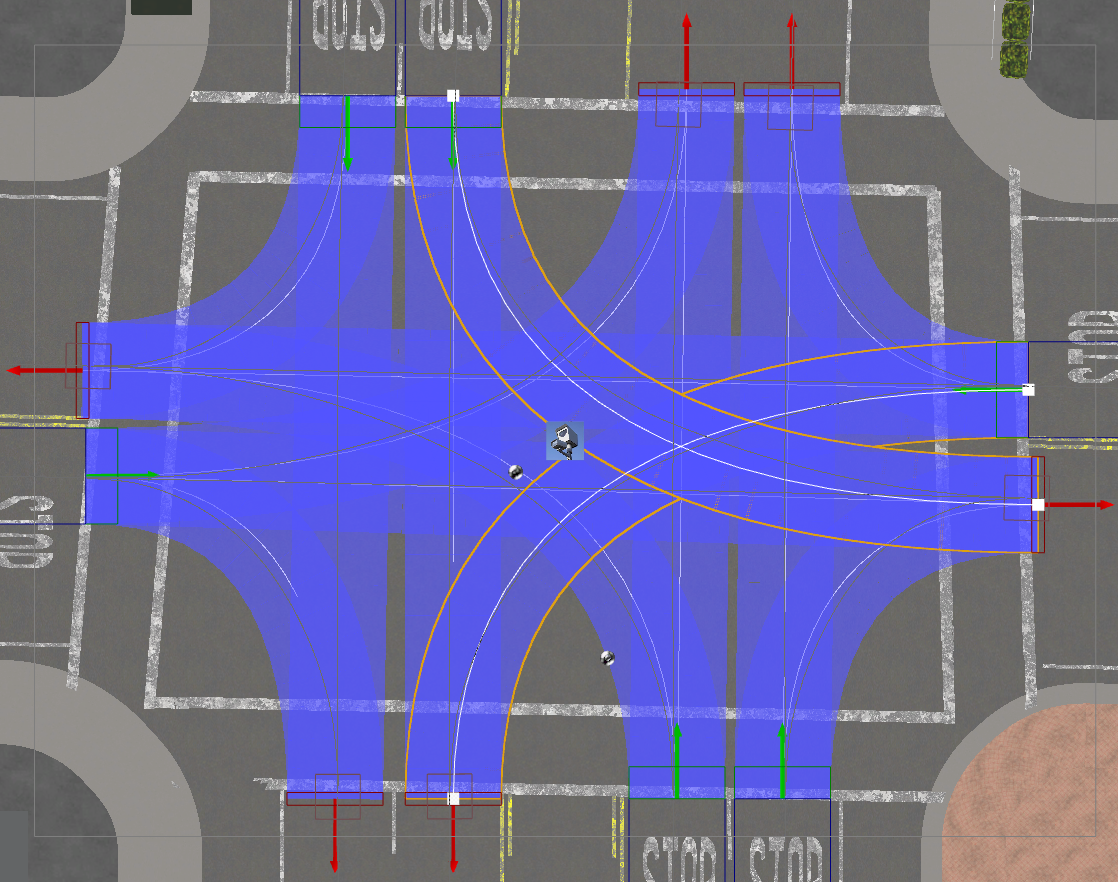
\includegraphics[width=0.5\linewidth]{figures/chapter3/lane_intersection.png}
\caption{Intersecting lanes.}
\label{fig:lane-intersection}
\vspace{-0.5cm}
\end{figure}
